%!TEX root = widefieldscan.tex
\svnidlong
{$HeadURL$}
{$LastChangedDate$}
{$LastChangedRevision$}
{$LastChangedBy$}
%
%\ifhtml
%\else
%\begin{center}
%	\fbox{
%		\begin{minipage}{.618\columnwidth}
%		The section below is versioned at \url{\svnkw{HeadURL}} (last commit @ \svnfileday.\svnfilemonth.\svnfileyear \space \svnfilehour:\svnfileminute, Revision: \svnkw{LastChangedRevision}).
%		\end{minipage}
%	} 
%\end{center}
%\fi
%
\section{Materials and Methods}%
\label{sec:materials and methods}%
\subsection{Sample Preparation and Image Acquisition}%
Rat lung samples, prepared according to %
\ifhtml
	\citet{Tschanz2002} and \citet{Luyet2002}
\else
	\citeasnoun{Tschanz2002} and \citeasnoun{Luyet2002}
\fi%
were used as test objects. Briefly, lungs of Sprague-Dawley rats were filled with \SI{2.5}{\percent} glutaraldehyde (C$_5$H$_8$O$_2$) in \SI{0.03}{\Molar} potassium-phosphate buffer (pH 7.4) by instillation via tracheotomy at a constant pressure of \SI{20}{\centi\meter} water column. In order to prevent a recoiling of the lung, the pressure was maintained during fixation (for a minimum of \SI{2}{\hour}). Subsequently, the lungs were dissected free and immersed in toto in the same fixative at a temperature of \SI{4}{\celsius} for at least \SI{24}{\hour}.

The samples were postfixed with \SI{1}{\percent} osmium tetroxide (OsO$_4$) and stained with \SI{4}{\percent} uranyl acetate (C$_4$H$_6$O$_6$U) to increase the x-ray absorption contrast, dehydrated in a graded series of ethanol and embedded in paraffin using Histoclear (Merck KGaA, Darmstadt, Germany) as an intermedium. The lung samples were mounted onto standard scanning electron microscopy sample holders (PLANO GmbH, Wetzlar, Germany) using paraffin.

The handling of animals before and during the experiments, as well as the experiments themselves, was approved and supervised by the Swiss Agency for the Environment, Forests and Landscape and the Veterinary Service of the Canton of Bern, Switzerland.

\subsection{SRXTM}%
The experiments were performed on the TOMCAT beamline~\cite{Stampanoni2006a} at the Swiss Light Source, Paul Scherrer Institut, Villigen, Switzerland. TOMCAT receives photons from a \SI{2.9}{\tesla} super-bending magnet with a critical energy of \SI{11.1}{\kilo\electronvolt} (corresponding to a wavelength of \SI{1.22}{\angstrom}). A double crystal multilayer monochromator covers an energy range between 6 and \SI{45}{\kilo\electronvolt}, with a bandwidth range of a few percent.

\subsubsection{Image acquisition and reconstruction}%
\label{seq:Image Acquisition}%
The samples were scanned at an x-ray energy of \SI{12.6}{\kilo\electronvolt}, which results in high contrast of the stained tissue to the paraffin, and thus a high signal to noise ratio. After penetration of the sample, the x-rays were converted into visible light by a YAG:Ce scintillator (\SI{18}{\micro\meter} thickness, Crismatec Saint-Gobain, Nemours, France). The projection images were magnified by diffraction limited microscope optics and digitized by a high-resolution 2048$\times$2048 pixel CCD camera (pco.2000, PCO AG, Kelheim, Germany) with 14 bit dynamic range. The lung samples were imaged using a 10$\times$ magnification, with 2$\times$2 binning and \SI{175}{\milli\second} exposure time resulting in isotropic voxels with a side length of \SI{1.48}{\micro\meter}.

Projection images $I_{Pr}$, essentially single radiographies of the sample, were recorded at several angular positions between \SI{0}{\degree} and \SI{180}{\degree}. The exact number of angular projections depended on the selected scan protocol, as described in section~\ref{subsec:quality-guided-protocols}. Additionally, a set of dark ($I_{D}$) and flat images ($I_{F}$) were recorded for each protocol. The dark images recorded at the start of the scan capture the noise and dark current of the camera. The flat images recorded at the start and at the end of the scan capture the beam profile and were used to baseline correct the raw projections.

Corrected projection images $I_{cPr}$ were obtained by correcting $I_{Pr}$ with the average dark ($\overline{I_{D}}$) and average flat image ($\overline{I_{F}}$) using the Beer-Lambert law (see below) and the relation described in equation~\ref{eq:cpr}.

The Beer--Lambert law relates the absorption of electromagnetic waves to the properties of the material through which the waves are traveling. Let $I_{0}$ and $I_{1}$ be the intensity of the incident electromagnetic wave and the intensity after penetration of the material, respectively. If $\mu$ describes the absorption coefficient of the substance and $l$ the path length that the wave travels through the material, then the intensity of the transmitted wave $I_{1}$ can be calculated using the Beer--Lambert law: \(I_{1}=I_{0}e^{-\mu l}\label{eq:beer-lambert}\). In general, $I_{0}$ and $\mu$ depend on the energy of the incident wave, so the equation only holds for a monochromatic beam, which is present at TOMCAT.

The recorded projections, i.e.\ the measured data, are defined as $I_{P}=\mu l=-ln\left(\frac{I_{1}}{I_{0}}\right)$, which corresponds to the inverse Beer--Lambert law. Using the dark and flat images, the corrected projection images $I_{cPr}$ have been calculated as follows:
\begin{equation}
	I_{cPr} = -ln\left(\frac{I_{Pr}-\overline{I_{D}}}{\overline{I_{F}}-\overline{I_{D}}}\right)
	= ln(\overline{I_{F}}-\overline{I_{D}})-ln(I_{Pr}-\overline{I_{D}})
	\label{eq:cpr}
\end{equation}

A detailed description of the workflow at TOMCAT and the steps necessary to compute a tomographic data set from a set of angular projections can be found in%
\ifhtml
	~\citet{Hintermueller2009}
\else
	~\citeasnoun{Hintermueller2009}
\fi%
.

\subsubsection{Covering a wide lateral field of view}%
For parallel beam geometry, tomographic images are obtained at equidistant angles over a sample rotation of \SI{180}{\degree} as shown in figure~\ref{fig:scanning-possibilities}(a). After reconstruction, the width of the image corresponds to the field of view of the camera.

Samples which are twice as large as the field of view can be imaged using scanning protocols based on a \SI{360}{\degree} off-center sample rotation as shown in figure~\ref{fig:scanning-possibilities}(b). Images recorded between \SI{180}{\degree} and \SI{360}{\degree} have to be flipped after acquisition, and the projection images obtained at position $I_{Pr_{x}}$ and $I_{Pr_{x+\SI{180}{\degree}}}$ are stitched together to projection images covering two times the field of view of the camera.

\ifiucr
	%\onecolumn
	\begin{figure}
		\centering
		\caption{Covering the field of view of differently sized samples with one \SI{180}{\degree} scan (a), one \SI{360}{\degree} scan (b) or---in the case of the so called wide field scanning---with multiple subscans (three subscans, c). The filled segments mark the region of the sample that is covered while scanning the respective positions (Position 1: red/checkerboard, Position 2: green, Position 3: blue/striped).}%
		%\documentclass{article}
%\usepackage[demo]{graphicx}
%\usepackage{subfig}
%\usepackage{tikz}
%\usepackage{multirow}
%\usepackage{siunitx}
%\begin{document}
%\begin{figure}
%%%%%%%%%%%%%%%%%%%%%%%%%%%%%
%\begin{tabular}{cc}
%Fig A & \multirow{3}{*}{Fig D}\\
%Fig B & \\
%Fig C & \\
%\end{tabular}
\noindent\makebox[\textwidth]{%
\begin{tabular}{cc}
%%%%% LEFT TOP %%%%%
	\subfloat[\SI{180}{\degree-scan}]{
		%%%%%
		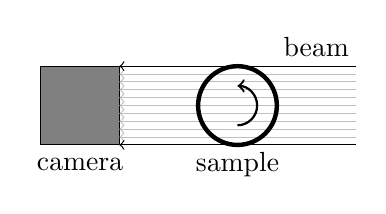
\begin{tikzpicture}
			%drawing grid
			%\draw[color=gray] (0,0) grid (8,1);
			\def\start{0}
			\def\length{1}
			%camera
			\draw [fill=gray] (\start,\start) rectangle (\length,\length);
			\node at (.5*\length,-.25) {camera};
			% beam
			\foreach \x in {0,.1,...,1.1}
				\draw[gray!50,<-] (\length,\x) -- (4*\length,\x);
			\foreach \x in {0,\length}
				\draw[<-] (\length,\x) -- (4*\length,\x);
			\node at (3.5*\length,\length+.25) {beam};
			%sample
			\draw[ultra thick] (2.5*\length,0.5*\length) circle (.5*\length);
			\draw[thick,->] (2.5*\length,0.25*\length) arc (-90:90:.25*\length);
			\node at (2.5*\length,-.25) {sample};
		\end{tikzpicture}
		%%%%%
		\label{subfig:180degreescan}
	}%
& %%%%% RIGHT TOP %%%%%
	\multirow{3}{*}{%
	\subfloat[Stacked scanning for long and thin samples]{
		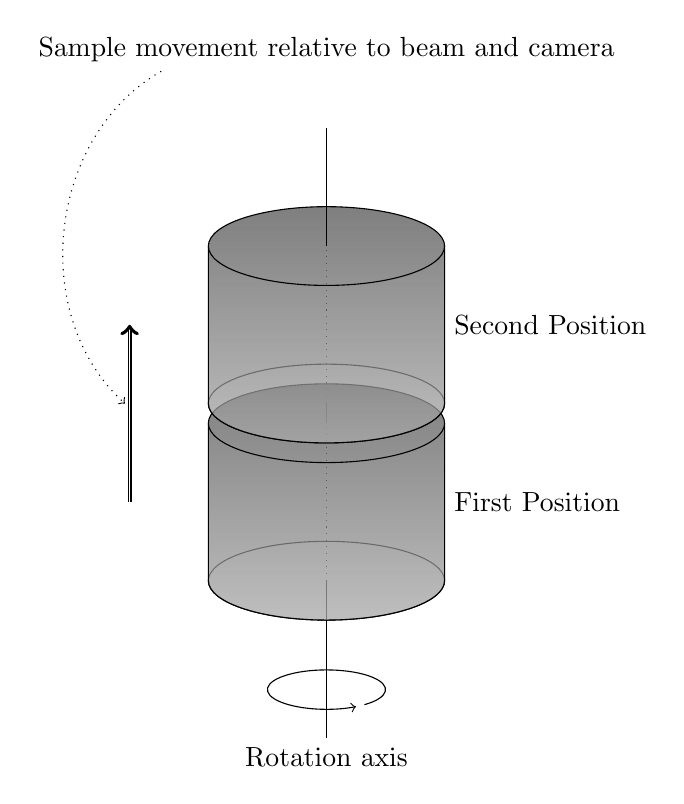
\begin{tikzpicture}%[ultra thick,scale=1]%,show background grid]
			%draw axes
				%\draw[ultra thick] (-10,0) -- (10,0);
				%\draw[ultra thick] (0,-10) -- (0,10);
				%\draw[ultra thick] (0,0) circle (.125);
			% rotation axis
				\draw[->] (0,-2) ++ (-50:.75) arc (-50:300:.75 and .25);
				\draw (0,-3) node [below] {Rotation axis} -- ++(0,2);
				\draw[dotted] (0,-1) -- ++(0,2);
				\draw (0,1) -- ++(0,0.25);
				\draw[dotted] (0,1.25) -- ++(0,2);
			% position 1
				\draw (0,-1) circle (1.5 and .5);
				\fill[shade,semitransparent] (-1.5,-1) arc (-180:0:1.5 and .5) -- ++(0,2) arc (0:180:1.5 and .5) -- cycle;
				\draw (-1.5,-1) arc (-180:0:1.5 and .5) -- ++(0,2) arc (0:180:1.5 and .5) -- cycle;		
				\draw (-1.5,1) arc (-180:0:1.5 and .5);
				\draw (1.5,0) node [right] {First Position};
			% position 2
				\draw (0,1.25) circle (1.5 and .5);
				\fill[shade,semitransparent] (-1.5,1.25) arc (-180:0:1.5 and .5) -- ++(0,2) arc (0:180:1.5 and .5) -- cycle;
				\draw (-1.5,1.25) arc (-180:0:1.5 and .5) -- ++(0,2) arc (0:180:1.5 and .5) -- cycle;		
				\draw (-1.5,3.25) arc (-180:0:1.5 and .5);
				\draw (1.5,2.25) node [right] {Second Position};
			% rotation axis on top
				\draw (0,3.25) -- ++(0,1.5);									
			% sample movement
				\draw[double,->] (-2.5,0) -- (-2.5,2.25) ;% node [text width=10cm,midway,left] {Sample movement relative to beam and camera};	
				% sample movement
				\node (movefrom) at (0,5.75) {Sample movement relative to beam and camera};
				\node (moveto) at (-2.5,1.125) {};
				\draw [->,dotted] (movefrom) to [bend right=54] (moveto);
		\end{tikzpicture}
		\label{subfig:stackedscan}
	}%
	}
\\
%%%%% LEFT MIDDLE %%%%%	
	\subfloat[\SI{360}{\degree-scan}]{
		%%%%%
		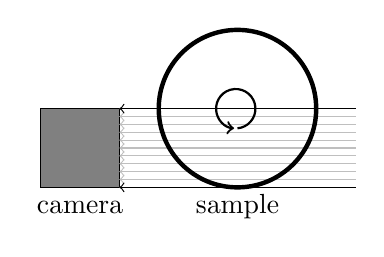
\begin{tikzpicture}
			%drawing grid
			%\draw[color=gray] (0,0) grid (8,1);
			\def\start{0}
			\def\length{1}
			%camera
			\draw [fill=gray] (\start,\start) rectangle (\length,\length);
			\node at (.5*\length,-.25) {camera};
			% beam
			\foreach \x in {0,.1,...,1.1}
				\draw[gray!50,<-] (\length,\x) -- (4*\length,\x);
			\foreach \x in {0,\length}
				\draw[<-] (\length,\x) -- (4*\length,\x);
		%	\node at (3.5*\length,\length+.25) {beam};
			%sample
			\draw[ultra thick] (2.5*\length,\length) circle (\length);
			\draw[thick,->] (2.5*\length,\length-0.25*\length) arc (-85:265:0.25*\length);
			\node at (2.5*\length,-.25) {sample};
		\end{tikzpicture}
		%%%%%
		\label{subfig:360degreescan}
	}%
& %%%%% RIGHT MIDDLE %%%%%
\\
%%%%% LEFT BOTTOMT %%%%%
	\subfloat[wide field scan]{
		%%%%%
		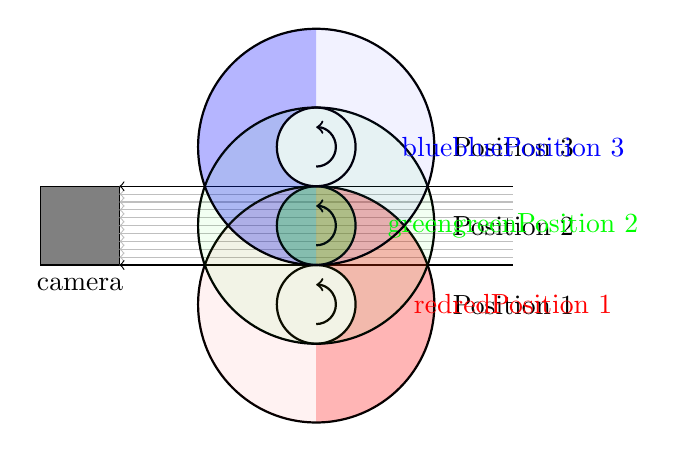
\begin{tikzpicture}
			\def\length{1}
			\def\beamlength{6}
			%grid
		%	\draw[color=gray] (0,-3) grid (7,3);
			%camera
			\draw [fill=gray] (0,0) rectangle (\length,\length);
			\node at (.5*\length,-.25) {camera};
			% beam
			\foreach \x in {0,.1,...,1.1}
				\draw[gray!50,<-] (\length,\x) -- (\beamlength,\x);
			\foreach \x in {0,\length}
				\draw[<-] (\length,\x) -- (\beamlength,\x);
		%	\node at (3.5*\length,\length+.25) {beam};
		%%%%%	%colored samples
		%%%%%	\foreach \y/\color/\position in {-.5/red/1,.5/green/2,1.5/blue/3}
		%%%%%		{
		%%%%%			\draw[thick,color=\color] (0.5*\beamlength+0.5*\length,\y) circle (1.5*\length) circle (.5*\length);
		%%%%%			\draw[thick,->,color=\color] (0.5*\beamlength+0.5*\length,\y-.25*\length) arc (-90:90:0.25*\length);
		%%%%%			\node[color=\color] at (\beamlength,\y) {Position \position};
		%%%%%		}
			% filled samples
			\fill [color=red,nearly transparent]   (3.5,1) arc (90:-90:1.5*\length) -- ++(0,1) arc (-90:90:.5*\length);
			\fill [color=blue,nearly transparent]  (3.5,3) arc (90:270:1.5*\length) -- ++(0,1) arc (270:90:.5*\length);
			\fill [color=green,nearly transparent] (0.5*\beamlength+0.5*\length,.5) circle (0.5*\length);	
			\foreach \y/\position/\color in {-.5/1/red,.5/2/green,1.5/3/blue}
				{
					\draw[thick] (0.5*\beamlength+0.5*\length,\y) circle (1.5*\length) circle (.5*\length);
					\draw[thick,->] (0.5*\beamlength+0.5*\length,\y-.25*\length) arc (-90:90:0.25*\length);
					\fill [color=\color,ultra nearly transparent] (0.5*\beamlength+0.5*\length,\y) circle (1.5*\length);
					\node at (\beamlength+.005,\y-.005) {Position \position};
					\node [color=\color] at (\beamlength,\y) {Position \position};
				}
		\end{tikzpicture}
		%%%%%
		\label{subfig:widefieldscan}
	}%
& %%%%% RIGHT BOTTOM %%%%%
\\
\end{tabular}
} %makebox
%%%%%%%%%%%%%%%%%%%%%%%%%%%%%	
%\caption{Caption of subfigures \subref{subfig:180degreescan}, \subref{subfig:360degreescan}, \subref{subfig:widefieldscan} and \subref{subfig:stackedscan}}
%\end{figure}
%\end{document}%
		\label{fig:scanning-possibilities}%
	\end{figure}
	%\twocolumn
\else
	\begin{figure}
		%\documentclass{article}
%\usepackage[demo]{graphicx}
%\usepackage{subfig}
%\usepackage{tikz}
%\usepackage{multirow}
%\usepackage{siunitx}
%\begin{document}
%\begin{figure}
%%%%%%%%%%%%%%%%%%%%%%%%%%%%%
%\begin{tabular}{cc}
%Fig A & \multirow{3}{*}{Fig D}\\
%Fig B & \\
%Fig C & \\
%\end{tabular}
\noindent\makebox[\textwidth]{%
\begin{tabular}{cc}
%%%%% LEFT TOP %%%%%
	\subfloat[\SI{180}{\degree-scan}]{
		%%%%%
		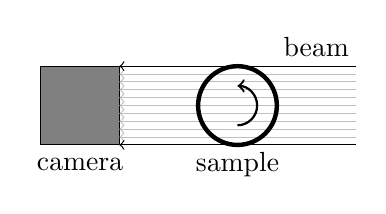
\begin{tikzpicture}
			%drawing grid
			%\draw[color=gray] (0,0) grid (8,1);
			\def\start{0}
			\def\length{1}
			%camera
			\draw [fill=gray] (\start,\start) rectangle (\length,\length);
			\node at (.5*\length,-.25) {camera};
			% beam
			\foreach \x in {0,.1,...,1.1}
				\draw[gray!50,<-] (\length,\x) -- (4*\length,\x);
			\foreach \x in {0,\length}
				\draw[<-] (\length,\x) -- (4*\length,\x);
			\node at (3.5*\length,\length+.25) {beam};
			%sample
			\draw[ultra thick] (2.5*\length,0.5*\length) circle (.5*\length);
			\draw[thick,->] (2.5*\length,0.25*\length) arc (-90:90:.25*\length);
			\node at (2.5*\length,-.25) {sample};
		\end{tikzpicture}
		%%%%%
		\label{subfig:180degreescan}
	}%
& %%%%% RIGHT TOP %%%%%
	\multirow{3}{*}{%
	\subfloat[Stacked scanning for long and thin samples]{
		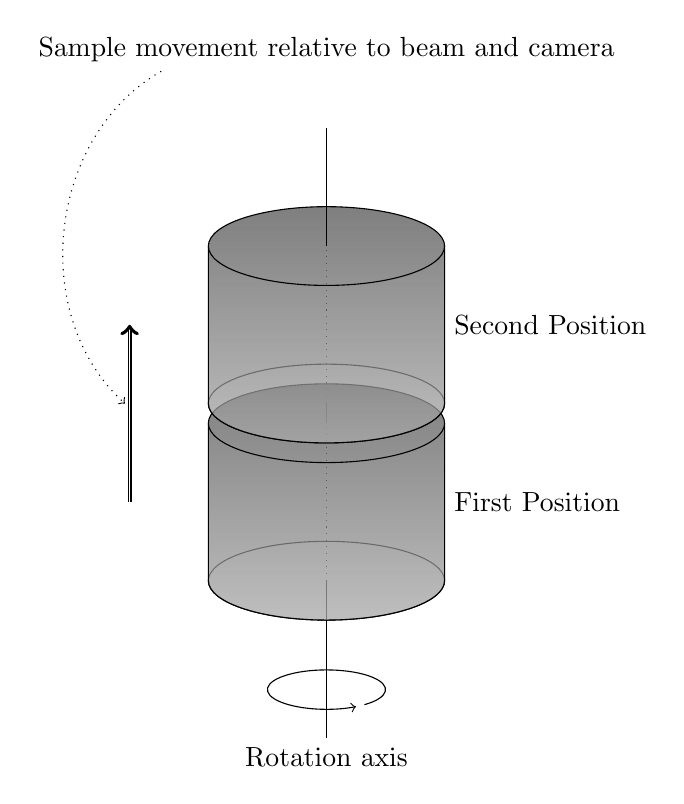
\begin{tikzpicture}%[ultra thick,scale=1]%,show background grid]
			%draw axes
				%\draw[ultra thick] (-10,0) -- (10,0);
				%\draw[ultra thick] (0,-10) -- (0,10);
				%\draw[ultra thick] (0,0) circle (.125);
			% rotation axis
				\draw[->] (0,-2) ++ (-50:.75) arc (-50:300:.75 and .25);
				\draw (0,-3) node [below] {Rotation axis} -- ++(0,2);
				\draw[dotted] (0,-1) -- ++(0,2);
				\draw (0,1) -- ++(0,0.25);
				\draw[dotted] (0,1.25) -- ++(0,2);
			% position 1
				\draw (0,-1) circle (1.5 and .5);
				\fill[shade,semitransparent] (-1.5,-1) arc (-180:0:1.5 and .5) -- ++(0,2) arc (0:180:1.5 and .5) -- cycle;
				\draw (-1.5,-1) arc (-180:0:1.5 and .5) -- ++(0,2) arc (0:180:1.5 and .5) -- cycle;		
				\draw (-1.5,1) arc (-180:0:1.5 and .5);
				\draw (1.5,0) node [right] {First Position};
			% position 2
				\draw (0,1.25) circle (1.5 and .5);
				\fill[shade,semitransparent] (-1.5,1.25) arc (-180:0:1.5 and .5) -- ++(0,2) arc (0:180:1.5 and .5) -- cycle;
				\draw (-1.5,1.25) arc (-180:0:1.5 and .5) -- ++(0,2) arc (0:180:1.5 and .5) -- cycle;		
				\draw (-1.5,3.25) arc (-180:0:1.5 and .5);
				\draw (1.5,2.25) node [right] {Second Position};
			% rotation axis on top
				\draw (0,3.25) -- ++(0,1.5);									
			% sample movement
				\draw[double,->] (-2.5,0) -- (-2.5,2.25) ;% node [text width=10cm,midway,left] {Sample movement relative to beam and camera};	
				% sample movement
				\node (movefrom) at (0,5.75) {Sample movement relative to beam and camera};
				\node (moveto) at (-2.5,1.125) {};
				\draw [->,dotted] (movefrom) to [bend right=54] (moveto);
		\end{tikzpicture}
		\label{subfig:stackedscan}
	}%
	}
\\
%%%%% LEFT MIDDLE %%%%%	
	\subfloat[\SI{360}{\degree-scan}]{
		%%%%%
		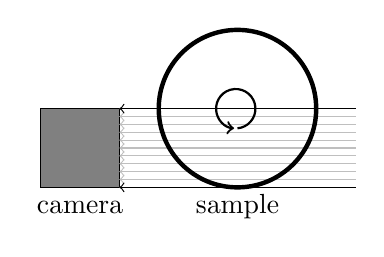
\begin{tikzpicture}
			%drawing grid
			%\draw[color=gray] (0,0) grid (8,1);
			\def\start{0}
			\def\length{1}
			%camera
			\draw [fill=gray] (\start,\start) rectangle (\length,\length);
			\node at (.5*\length,-.25) {camera};
			% beam
			\foreach \x in {0,.1,...,1.1}
				\draw[gray!50,<-] (\length,\x) -- (4*\length,\x);
			\foreach \x in {0,\length}
				\draw[<-] (\length,\x) -- (4*\length,\x);
		%	\node at (3.5*\length,\length+.25) {beam};
			%sample
			\draw[ultra thick] (2.5*\length,\length) circle (\length);
			\draw[thick,->] (2.5*\length,\length-0.25*\length) arc (-85:265:0.25*\length);
			\node at (2.5*\length,-.25) {sample};
		\end{tikzpicture}
		%%%%%
		\label{subfig:360degreescan}
	}%
& %%%%% RIGHT MIDDLE %%%%%
\\
%%%%% LEFT BOTTOMT %%%%%
	\subfloat[wide field scan]{
		%%%%%
		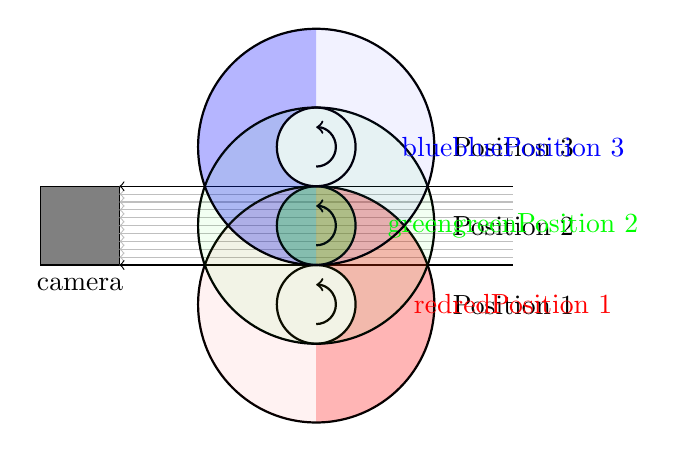
\begin{tikzpicture}
			\def\length{1}
			\def\beamlength{6}
			%grid
		%	\draw[color=gray] (0,-3) grid (7,3);
			%camera
			\draw [fill=gray] (0,0) rectangle (\length,\length);
			\node at (.5*\length,-.25) {camera};
			% beam
			\foreach \x in {0,.1,...,1.1}
				\draw[gray!50,<-] (\length,\x) -- (\beamlength,\x);
			\foreach \x in {0,\length}
				\draw[<-] (\length,\x) -- (\beamlength,\x);
		%	\node at (3.5*\length,\length+.25) {beam};
		%%%%%	%colored samples
		%%%%%	\foreach \y/\color/\position in {-.5/red/1,.5/green/2,1.5/blue/3}
		%%%%%		{
		%%%%%			\draw[thick,color=\color] (0.5*\beamlength+0.5*\length,\y) circle (1.5*\length) circle (.5*\length);
		%%%%%			\draw[thick,->,color=\color] (0.5*\beamlength+0.5*\length,\y-.25*\length) arc (-90:90:0.25*\length);
		%%%%%			\node[color=\color] at (\beamlength,\y) {Position \position};
		%%%%%		}
			% filled samples
			\fill [color=red,nearly transparent]   (3.5,1) arc (90:-90:1.5*\length) -- ++(0,1) arc (-90:90:.5*\length);
			\fill [color=blue,nearly transparent]  (3.5,3) arc (90:270:1.5*\length) -- ++(0,1) arc (270:90:.5*\length);
			\fill [color=green,nearly transparent] (0.5*\beamlength+0.5*\length,.5) circle (0.5*\length);	
			\foreach \y/\position/\color in {-.5/1/red,.5/2/green,1.5/3/blue}
				{
					\draw[thick] (0.5*\beamlength+0.5*\length,\y) circle (1.5*\length) circle (.5*\length);
					\draw[thick,->] (0.5*\beamlength+0.5*\length,\y-.25*\length) arc (-90:90:0.25*\length);
					\fill [color=\color,ultra nearly transparent] (0.5*\beamlength+0.5*\length,\y) circle (1.5*\length);
					\node at (\beamlength+.005,\y-.005) {Position \position};
					\node [color=\color] at (\beamlength,\y) {Position \position};
				}
		\end{tikzpicture}
		%%%%%
		\label{subfig:widefieldscan}
	}%
& %%%%% RIGHT BOTTOM %%%%%
\\
\end{tabular}
} %makebox
%%%%%%%%%%%%%%%%%%%%%%%%%%%%%	
%\caption{Caption of subfigures \subref{subfig:180degreescan}, \subref{subfig:360degreescan}, \subref{subfig:widefieldscan} and \subref{subfig:stackedscan}}
%\end{figure}
%\end{document}%
		\label{subfig:scanning-possibilities}%
		\caption{Covering the field of view of differently sized samples with one \SI{180}{\degree} scan (a), one \SI{360}{\degree} scan (b) or---in the case of the so called wide field scanning---with multiple subscans (three subscans, c). The filled segments mark the region of the sample that is covered while scanning the respective positions (Position 1: red/checkerboard, Position 2: green, Position 3: blue/striped).}%
		\label{fig:scanning-possibilities}%
	\end{figure}
\fi

If a tomographic scan covering a size wider than two field of views is desired, three or more \SI{180}{\degree} scans taken at slightly overlapping positions, as shown figure~\ref{fig:scanning-possibilities}(c) have to be combined. The projection images of each subscan overlap each other slightly to allow an optimal stitching of the multiple projections of each rotational angle into one projection. Using the mean squared difference between adjacent subscan images~\cite{Hintermueller2009}, such a cutline was calculated for the adjacent subscans and used to merge the single projections into projections covering the full field of view.

\subsection{Generation of multiple scanning protocols}%
The discussed scanning protocol for covering a wide field of view with three subscans is based on the assumption that a sufficient resolution and contrast can be achieved in the tomographic dataset, if the sampling theorem is individually fulfilled for each of the subscans. This results in a set of $i$ subscans with $P_{i}$ projection images. A simple example with $P_{1}=4$ and $P_{2}=P_{3}=8$ is shown in figure~\ref{fig:projections}(a).

To be able to reconstruct the sample, we need to stitch the individual sets of projections to projections spanning the desired field of view. Since each subscan has a different number of projections $P_{i}$, a stitching algorithm has to interpolate projections from adjacent projections (dashed lines in figure~\ref{fig:projections}(b)). Alternatively, an equal amount of projections have to be acquired for all subscans, leading to oversampling for the central scanning position.

\ifiucr
	\begin{figure}%
		\caption{Setup with three \SI{180}{\degree} scans; one central (green) and two lateral (red and blue, respectively). In this drawing, we chose four projections for the central and eight projections for each of the lateral scans. The colors of the three positions correspond to the colors shown in figure~\ref{fig:scanning-possibilities}(c). Panel a): scanned projections, panel b): scanned projections and additional interpolated projections (dashed) required to merge all projections.}%
		%\documentclass{article}
%\usepackage[demo]{graphicx}
%\usepackage{subfig}
%\usepackage{tikz}
%\usepackage{multirow}
%\usepackage{siunitx}
%\begin{document}
%\begin{figure}
%\centering
%%%%%%%%%%%%%%%%%%%%%%%%%%%%%
\def\radius{1}%
\def\gap{0.05}%
\begin{tikzpicture}[ultra thick,scale=.618]%
	\foreach \ang in {0,45,...,359}%
		{%
		\draw [color=green] (\ang:0) -- (\ang:\radius);%
		}%
	\foreach \ang in {0,22.5,...,179}%
		{%
		\draw [color=red] (\ang:\radius+\gap) -- (\ang:3*\radius+\gap);%
		}%
	\foreach \ang in {180,202.5,...,359}%
		{%
		\draw [color=blue] (\ang:\radius+\gap) -- (\ang:3*\radius+\gap);%
		}%
	\node [anchor=south west] at (-3.05,-3.05) {(a)};
\end{tikzpicture}
%%%%%%%%%%%%%%%%%%%%%%%%%%%%%	
%\caption{Projection Setup}
%\end{figure}
%\end{document}%
		\input{tikz-images/ProjectionSetupInterpolate}%
		\label{fig:projections}%
	\end{figure}%
\else
	\begin{figure*}[htp]
		\centering
		%\documentclass{article}
%\usepackage[demo]{graphicx}
%\usepackage{subfig}
%\usepackage{tikz}
%\usepackage{multirow}
%\usepackage{siunitx}
%\begin{document}
%\begin{figure}
%\centering
%%%%%%%%%%%%%%%%%%%%%%%%%%%%%
\def\radius{1}%
\def\gap{0.05}%
\begin{tikzpicture}[ultra thick,scale=.618]%
	\foreach \ang in {0,45,...,359}%
		{%
		\draw [color=green] (\ang:0) -- (\ang:\radius);%
		}%
	\foreach \ang in {0,22.5,...,179}%
		{%
		\draw [color=red] (\ang:\radius+\gap) -- (\ang:3*\radius+\gap);%
		}%
	\foreach \ang in {180,202.5,...,359}%
		{%
		\draw [color=blue] (\ang:\radius+\gap) -- (\ang:3*\radius+\gap);%
		}%
	\node [anchor=south west] at (-3.05,-3.05) {(a)};
\end{tikzpicture}
%%%%%%%%%%%%%%%%%%%%%%%%%%%%%	
%\caption{Projection Setup}
%\end{figure}
%\end{document}%
		\input{tikz-images/ProjectionSetupInterpolate}%
		\caption{Setup with three \SI{180}{\degree} scans; one central (green) and two lateral (red and blue, respectively). In this drawing, we chose four projections for the central and eight projections for each of the lateral scans. The colors of the three positions correspond to the colors shown in figure~\ref{fig:scanning-possibilities}(c). Panel a): scanned projections, panel b): scanned projections and additional interpolated projections (dashed) required to merge all projections.}%
		\label{fig:projections}
	\end{figure*}
\fi

\subsubsection{Reduction of acquisition time}\label{subsubsec:reduction-of-acquisition-time}%
Since the total acquisition time per sample linearly scales with the total amount of recorded projections for all subscans, we tend to avoid oversampling, to reduce the total amount of beam time used for one sample. Our goal was to find a good compromise between scanning and processing time, and image quality. In order to reduce the time required for scanning one sample, acquisition protocols with varying number of projections for each of the three subscans were designed.

To simplify the interpolation and merging of the projections from each subscan, we selected protocols where the fraction of the amount of projections of the inner ($P_{inner}$) to the outer subscans ($P_{outer}$) is always a multiple of two%: $\frac{P_{outer}}{P_{inner}} \bmod 2 = 0$
. In the simple case shown in figure~\ref{fig:projections}, we would acquire 4 projections for the central and 8 projections for each of the lateral scans, thus avoiding oversampling the central part of the sample. To be able to merge the projection images, we need to interpolate 4 projections (dashed) prior to stitching. If the number of projections acquired for the ring scans was not two times the number of projections of the central scan, the stitching of the projections would introduce additional processing steps to interpolate the required intermediate projections.

To be able to further reduce the total scanning time, we developed different scanning protocols related to a gold standard protocol, which per definition would cover the desired field of view while fulfilling the sampling theorem in all parts of the field of view, as shown in figure~\ref{fig:SubScan-Setup}(a). For this example, we would like to achieve a field of view of 3072 pixels. The dark gray circle, shown in the aforementioned figure is the field of view that can be fully covered. The rest of the slice (in light grey) would be either missing or show artifacts, depending on the chosen reconstruction algorithm. With a detector of the size of 1024$\times$1024 pixels, we could cover this field of view with nine independent scans. This would require nine independent reconstructions and stitching of those nine tomographic datasets into one dataset covering the full field of view. However, we could also cover the chosen field of view using a detector of the size of 3072$\times$1024 pixels in one scan. Using a scanning protocol with three subscans from which we obtain merged projections, we can cover the desired field of view using a much smaller detector. Figure~\ref{fig:SubScan-Setup}(b) shows how the desired field of view of 3072 pixels can be covered with a wide-field scan, composed of one central and two half ring-scans, recorded with a detector with a size of 1024$\times$1024 pixels. A further increase in the field of view can be obtained by simple iteration. Figures~\ref{fig:SubScan-Setup}(c)--(f) show such a setup for a five- or seven-fold increase.

\ifiucr
	\begin{figure}%
		\centering%
		\caption{Setup for different field of views. %
		(a) Desired field of view of 3072 pixel diameter. %
		(b) Gold standard scanning protocol for covering the desired field of view of panel (a) with merged projections from one central and two half ring scans ($r_{1}$ and $r_{2}$). %
		(c) Desired field of view of 5120 pixel diameter. %
		(d) Gold standard scanning protocol for covering the desired field of view of panel (c) with merged projections from one central and four half ring scans ($r_{1}$--$r_{4}$). %
		(e) Desired field of view of 7168 pixel diameter. %
		(f) Gold standard scanning protocol for covering the desired field of view of panel (e) with merged projections from one central and six half ring scans ($r_{1}$--$r_{6}$).%
		}%
		%\documentclass{article}
%\usepackage{subfig}
%\usepackage{tikz}
%\begin{document}
%\begin{figure}
%\centering
%%%%%%%%%%%%%%%%%%%%%%%%%%%%% 3 SUBSCANS %%%%%%%%%%%%%%%%%%%%%%%%%%%%%
\def\width{2.2}
\def\size{3}%
\def\scale{\width/\size}
	\begin{tikzpicture}[scale=\scale]
	%	\draw [dashed] (-1,-1) grid (7,7);
		\draw [fill=gray!25] (0,0) rectangle (2*\size,2*\size);
		\fill [semitransparent] (\size,\size) circle (\size);
		\draw (\size,\size) circle (\size);
		\draw [white,ultra thick,<->] (0,\size) -- node [above] {3072 px} (2*\size,\size);
		\node [anchor=south west] at (0,0) {(a)};%
	%	\draw [step=2] (0,0) grid (6,6);
	\end{tikzpicture}%
%	\hfill%
	\begin{tikzpicture}[scale=\scale]
%		\draw [dashed] (-1,-1) grid (7,7);
		\draw [fill=gray!25] (0,0) rectangle (2*\size,2*\size);
		\fill [semitransparent] (\size,\size) circle (\size);
		\foreach \r in {1,3}
			\draw (\size,\size) circle (\r);
		\draw (0,\size) -- (\size-1,\size);
		\draw (\size+1,\size) -- (2*\size,\size);
		\node at (\size,1) {$r_{1}$};
		\node at (\size,3) {central};
		\node at (\size,5) {$r_{2}$};
		\def\angle{155}
		\draw [white,ultra thick,<->] (\size,\size) +(\angle:1) -- node [sloped,midway,above] {1024 px} +(\angle:3); 
		\node [anchor=south west] at (0,0) {(b)};%
	\end{tikzpicture}%
%%%%%%%%%%%%%%%%%%%%%%%%%%%%% 3 SUBSCANS
%\\%
%%%%%%%%%%%%%%%%%%%%%%%%%%%%% 5 SUBSCANS
\def\size{5}%
\def\scale{\width/\size}
	\begin{tikzpicture}[scale=\scale]%
	%	\draw [dashed] (-1,-1) grid (7,7);
		\draw [fill=gray!25] (0,0) rectangle (2*\size,2*\size);
		\fill [semitransparent] (\size,\size) circle (\size);
		\draw (\size,\size) circle (\size);
		\draw [white,ultra thick,<->] (0,\size) -- node [above] {5120 px} (2*\size,\size);
		\node [anchor=south west] at (0,0) {(c)};%
	%	\draw [step=2] (0,0) grid (6,6);
	\end{tikzpicture}%
%	\hfill%
	\begin{tikzpicture}[scale=\scale]
%		\draw [dashed] (-1,-1) grid (7,7);
		\draw [fill=gray!25] (0,0) rectangle (2*\size,2*\size);
		\fill [semitransparent] (\size,\size) circle (\size);
		\foreach \r in {1,3,5}
			\draw (\size,\size) circle (\r);
		\draw (0,\size) -- (\size-1,\size);
		\draw (\size+1,\size) -- (2*\size,\size);
		\node at (\size,1) {$r_{3}$};
		\node at (\size,3) {$r_{1}$};
		\node at (\size,5) {central};
		\node at (\size,7) {$r_{2}$};
		\node at (\size,9) {$r_{4}$};
		\def\angle{155}
		\draw [white,ultra thick,<->] (\size,\size) +(\angle:1) -- node [sloped,midway,above] {1024 px} +(\angle:3); 
		\node [anchor=south west] at (0,0) {(d)};%
	\end{tikzpicture}%
%%%%%%%%%%%%%%%%%%%%%%%%%%%%% 5 SUBSCANS
%\\%
%%%%%%%%%%%%%%%%%%%%%%%%%%%%% 7 SUBSCANS
\def\size{7}%
\def\scale{\width/\size}
	\begin{tikzpicture}[scale=\scale]%
	%	\draw [dashed] (-1,-1) grid (7,7);
		\draw [fill=gray!25] (0,0) rectangle (2*\size,2*\size);
		\fill [semitransparent] (\size,\size) circle (\size);
		\draw (\size,\size) circle (\size);
		\draw [white,ultra thick,<->] (0,\size) -- node [above] {7168 px} (2*\size,\size);
	%	\draw [step=2] (0,0) grid (6,6);
		\node [anchor=south west] at (0,0) {(e)};%
	\end{tikzpicture}%
%	\hfill%
	\begin{tikzpicture}[scale=\scale]
%		\draw [dashed] (-1,-1) grid (7,7);
		\draw [fill=gray!25] (0,0) rectangle (2*\size,2*\size);
		\fill [semitransparent] (\size,\size) circle (\size);
		\foreach \r in {1,3,5,7}
			\draw (\size,\size) circle (\r);
		\draw (0,\size) -- (\size-1,\size);
		\draw (\size+1,\size) -- (2*\size,\size);
		\node at (\size,1) {$r_{5}$};
		\node at (\size,3) {$r_{3}$};
		\node at (\size,5) {$r_{1}$};
		\node at (\size,7) {central};
		\node at (\size,9) {$r_{2}$};
		\node at (\size,11) {$r_{4}$};
		\node at (\size,13) {$r_{6}$};
		\def\angle{155}
		\draw [white,ultra thick,<->] (\size,\size) +(\angle:1) -- node [sloped,midway,above] {1024 px} +(\angle:3);
		\node [anchor=south west] at (0,0) {(f)};%
	\end{tikzpicture}%
%%%%%%%%%%%%%%%%%%%%%%%%%%%%% 7 SUBSCANS %%%%%%%%%%%%%%%%%%%%%%%%%%%%%
%\\
%%%%%%%%%%%%%%%%%%%%%%%%%%%%%	
%\caption{Projection Setup}
%\end{figure}
%\end{document}
		\label{fig:SubScan-Setup}%
	\end{figure}%
\else
	\begin{figure*}[htp]
		\centering%
		%\documentclass{article}
%\usepackage{subfig}
%\usepackage{tikz}
%\begin{document}
%\begin{figure}
%\centering
%%%%%%%%%%%%%%%%%%%%%%%%%%%%% 3 SUBSCANS %%%%%%%%%%%%%%%%%%%%%%%%%%%%%
\def\width{2.2}
\def\size{3}%
\def\scale{\width/\size}
	\begin{tikzpicture}[scale=\scale]
	%	\draw [dashed] (-1,-1) grid (7,7);
		\draw [fill=gray!25] (0,0) rectangle (2*\size,2*\size);
		\fill [semitransparent] (\size,\size) circle (\size);
		\draw (\size,\size) circle (\size);
		\draw [white,ultra thick,<->] (0,\size) -- node [above] {3072 px} (2*\size,\size);
		\node [anchor=south west] at (0,0) {(a)};%
	%	\draw [step=2] (0,0) grid (6,6);
	\end{tikzpicture}%
%	\hfill%
	\begin{tikzpicture}[scale=\scale]
%		\draw [dashed] (-1,-1) grid (7,7);
		\draw [fill=gray!25] (0,0) rectangle (2*\size,2*\size);
		\fill [semitransparent] (\size,\size) circle (\size);
		\foreach \r in {1,3}
			\draw (\size,\size) circle (\r);
		\draw (0,\size) -- (\size-1,\size);
		\draw (\size+1,\size) -- (2*\size,\size);
		\node at (\size,1) {$r_{1}$};
		\node at (\size,3) {central};
		\node at (\size,5) {$r_{2}$};
		\def\angle{155}
		\draw [white,ultra thick,<->] (\size,\size) +(\angle:1) -- node [sloped,midway,above] {1024 px} +(\angle:3); 
		\node [anchor=south west] at (0,0) {(b)};%
	\end{tikzpicture}%
%%%%%%%%%%%%%%%%%%%%%%%%%%%%% 3 SUBSCANS
%\\%
%%%%%%%%%%%%%%%%%%%%%%%%%%%%% 5 SUBSCANS
\def\size{5}%
\def\scale{\width/\size}
	\begin{tikzpicture}[scale=\scale]%
	%	\draw [dashed] (-1,-1) grid (7,7);
		\draw [fill=gray!25] (0,0) rectangle (2*\size,2*\size);
		\fill [semitransparent] (\size,\size) circle (\size);
		\draw (\size,\size) circle (\size);
		\draw [white,ultra thick,<->] (0,\size) -- node [above] {5120 px} (2*\size,\size);
		\node [anchor=south west] at (0,0) {(c)};%
	%	\draw [step=2] (0,0) grid (6,6);
	\end{tikzpicture}%
%	\hfill%
	\begin{tikzpicture}[scale=\scale]
%		\draw [dashed] (-1,-1) grid (7,7);
		\draw [fill=gray!25] (0,0) rectangle (2*\size,2*\size);
		\fill [semitransparent] (\size,\size) circle (\size);
		\foreach \r in {1,3,5}
			\draw (\size,\size) circle (\r);
		\draw (0,\size) -- (\size-1,\size);
		\draw (\size+1,\size) -- (2*\size,\size);
		\node at (\size,1) {$r_{3}$};
		\node at (\size,3) {$r_{1}$};
		\node at (\size,5) {central};
		\node at (\size,7) {$r_{2}$};
		\node at (\size,9) {$r_{4}$};
		\def\angle{155}
		\draw [white,ultra thick,<->] (\size,\size) +(\angle:1) -- node [sloped,midway,above] {1024 px} +(\angle:3); 
		\node [anchor=south west] at (0,0) {(d)};%
	\end{tikzpicture}%
%%%%%%%%%%%%%%%%%%%%%%%%%%%%% 5 SUBSCANS
%\\%
%%%%%%%%%%%%%%%%%%%%%%%%%%%%% 7 SUBSCANS
\def\size{7}%
\def\scale{\width/\size}
	\begin{tikzpicture}[scale=\scale]%
	%	\draw [dashed] (-1,-1) grid (7,7);
		\draw [fill=gray!25] (0,0) rectangle (2*\size,2*\size);
		\fill [semitransparent] (\size,\size) circle (\size);
		\draw (\size,\size) circle (\size);
		\draw [white,ultra thick,<->] (0,\size) -- node [above] {7168 px} (2*\size,\size);
	%	\draw [step=2] (0,0) grid (6,6);
		\node [anchor=south west] at (0,0) {(e)};%
	\end{tikzpicture}%
%	\hfill%
	\begin{tikzpicture}[scale=\scale]
%		\draw [dashed] (-1,-1) grid (7,7);
		\draw [fill=gray!25] (0,0) rectangle (2*\size,2*\size);
		\fill [semitransparent] (\size,\size) circle (\size);
		\foreach \r in {1,3,5,7}
			\draw (\size,\size) circle (\r);
		\draw (0,\size) -- (\size-1,\size);
		\draw (\size+1,\size) -- (2*\size,\size);
		\node at (\size,1) {$r_{5}$};
		\node at (\size,3) {$r_{3}$};
		\node at (\size,5) {$r_{1}$};
		\node at (\size,7) {central};
		\node at (\size,9) {$r_{2}$};
		\node at (\size,11) {$r_{4}$};
		\node at (\size,13) {$r_{6}$};
		\def\angle{155}
		\draw [white,ultra thick,<->] (\size,\size) +(\angle:1) -- node [sloped,midway,above] {1024 px} +(\angle:3);
		\node [anchor=south west] at (0,0) {(f)};%
	\end{tikzpicture}%
%%%%%%%%%%%%%%%%%%%%%%%%%%%%% 7 SUBSCANS %%%%%%%%%%%%%%%%%%%%%%%%%%%%%
%\\
%%%%%%%%%%%%%%%%%%%%%%%%%%%%%	
%\caption{Projection Setup}
%\end{figure}
%\end{document}
		\caption{Setup for different field of views. %
		(a) Desired field of view of 3072 pixel diameter. %
		(b) Gold standard scanning protocol for covering the desired field of view of panel (a) with merged projections from one central and two half ring scans ($r_{1}$ and $r_{2}$). %
		(c) Desired field of view of 5120 pixel diameter. %
		(d) Gold standard scanning protocol for covering the desired field of view of panel (c) with merged projections from one central and four half ring scans ($r_{1}$--$r_{4}$). %
		(e) Desired field of view of 7168 pixel diameter. %
		(f) Gold standard scanning protocol for covering the desired field of view of panel (e) with merged projections from one central and six half ring scans ($r_{1}$--$r_{6}$).%
		}%
		\label{fig:SubScan-Setup}%
	\end{figure*}
\fi

\subsection{Wide Field Scanning Pipeline}%
\label{subsec:wfs-setup}%
A MATLAB-script (MATLAB\textsuperscript{\textregistered} 7.6.0.321 (R2008a), The MathWorks, Inc.) reads several parameters like desired field of view, detector width, magnification and binning and calculates the number of projections needed to satisfy the sampling theorem for the chosen field of view. This gold-standard protocol is used to compute a set of acquisition protocols with reduced amount of projections.

Using a Shepp-Logan phantom~\cite{Shepp1974}, a reconstruction is calculated for each protocol of this set. The expected reconstruction quality is calculated, based on the difference between the simulated reconstructions and the gold standard (the original phantom). This calculated reconstruction quality is then plotted against the acquisition time, which enables the user to chose a suitable protocol balancing image quality and acquisition time.

After the user has chosen a suitable protocol out of the presented set, a file containing the details of the scan is written to disk. This file contains the parameters needed to scan this protocol: the number of required subscans, the positions of the sample, the number of projections and the start and stop angles of the rotation for each subscan. A custom Python-script (\url{http://python.org/}) parses the file containing the details and interacts with the EPICS-System (Experimental Physics and Industrial Control System, Argonne National Laboratory, Argonne, USA, \url{http://www.aps.anl.gov/epics/}), which itself is used to control the hardware of the TOMCAT beamline, enabling an unattended batch scan of all the desired subscans.

After the multiple subscans have been recorded, the stitching of the projections recorded per subscans into projections covering the desired field of view is performed with minimal user interaction using a second MATLAB-script. Further processing of the merged projections such as sinogram generation and reconstruction into the tomographic dataset are integrated into the TOMCAT data-processing pipeline, as specified by%
\ifhtml%
	~\citet{Hintermueller2009}%
\else%
	~\citeasnoun{Hintermueller2009}%
\fi%
.

\subsection{Batch Acquisition of the Protocols}%
Multiple scanning protocols were defined. The total amount of recorded projections for the different protocols were linearly scaled down compared to a gold standard scan (for details, see section~\ref{subsec:quality-guided-protocols}). All parameters of each protocol, such as sample-position in relation to the beam, rotation angles and amount of projections to obtain for each of the individual subscans were set in a preference-file, generated using the aforementioned MATLAB-script. All 19 protocols (B--T) were scanned as a batch scan without manual intervention, permitting a direct comparison of the reconstructed datasets.

After acquisition of the three subscans per protocol, custom MATLAB functions read the parameters of the single subscans (e.g.\ sample name, amount of subscans, amount of dark and flat images) as well as the desired output-name and -suffix, and performed all necessary calculations, including: loading of the correct projections from each subscan; normalizing; interpolation; cutline detection; correct stitching of the images into wide field projections, and; writing these projections to disk.

The merged projections were rearranged into sinograms, where the $n$\textsuperscript{th} is composed of the $n$\textsuperscript{th} line of every corrected projection. The $n$\textsuperscript{th} slice of the tomographic scan was reconstructed from the $n$\textsuperscript{th} sinogram using an FFT-based regridding algorithm~\cite{Dowd1999}. The 19 tomographic datasets were reconstructed on a 20-node server farm (five \SI{64}{\bit} Opteron machines with 4 cores and \SI{8}{\giga\byte} RAM each). The reconstructions resulted in an image stack covering a large sample volume of 2793$\times$2793$\times$1024 pixels, an approximately nine-fold increase from the standard volume of 1024$\times$1024$\times$1024 pixels for one conventional scan.